\documentclass{standalone}
\usepackage{tikz}
\usetikzlibrary{patterns}
\usetikzlibrary{positioning}
\usetikzlibrary{patterns, positioning}
\usetikzlibrary{shapes.misc}
\usepackage[outline]{contour}
\contourlength{1.5pt} 
\usetikzlibrary{calc}
        \usepackage{relsize}
        \tikzset{fontscale/.style = {font=\relsize{#1}}}

\begin{document}
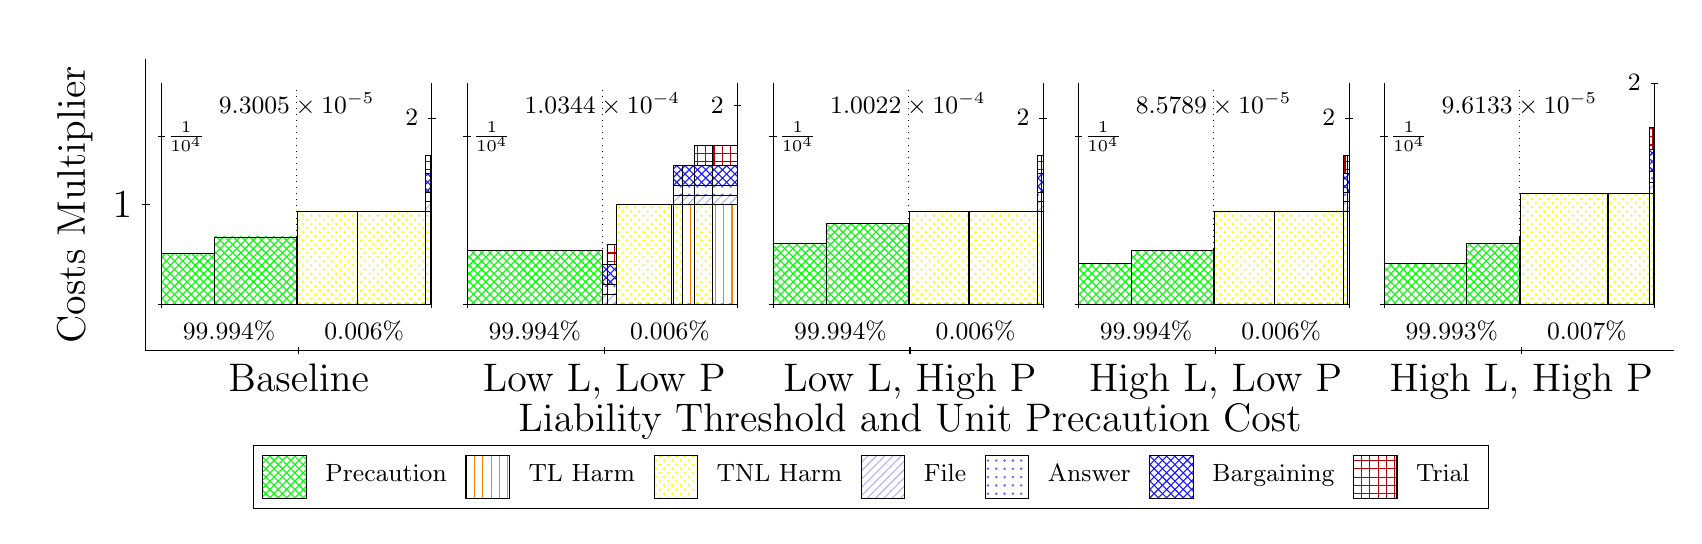
\begin{tikzpicture}
\clip(-0.5,-1.1) rectangle +(20.91,6.2);
\draw[black] (1,1) -- (1,4.7);
\node[rotate=90, fontscale=2, anchor=center] at (0.1, 2.85) {Costs Multiplier};
\draw[black] (0.95,2.85) -- (1.05,2.85);
\node[fontscale=2, anchor=east] at (0.95, 2.85) {1};

\draw[black] (1,1) -- (20.41,1);
\node[fontscale=2, anchor=center] at (10.705, 0.1) {Liability Threshold and Unit Precaution Cost};
\draw[black] (2.941,0.95) -- (2.941,1.05);
\node[fontscale=2, anchor=north] at (2.941, 0.95) {Baseline};
\draw[black] (6.823,0.95) -- (6.823,1.05);
\node[fontscale=2, anchor=north] at (6.823, 0.95) {Low L, Low P};
\draw[black] (10.705,0.95) -- (10.705,1.05);
\node[fontscale=2, anchor=north] at (10.705, 0.95) {Low L, High P};
\draw[black] (14.587,0.95) -- (14.587,1.05);
\node[fontscale=2, anchor=north] at (14.587, 0.95) {High L, Low P};
\draw[black] (18.469,0.95) -- (18.469,1.05);
\node[fontscale=2, anchor=north] at (18.469, 0.95) {High L, High P};


\draw[pattern=crosshatch, pattern color=green,draw=black,very thin] (1.2,1.592) rectangle (1.8725,2.2292);
\draw[pattern=crosshatch, pattern color=green,draw=black,very thin] (1.8725,1.592) rectangle (2.916,2.4416);
\draw[pattern=crosshatch, pattern color=green,draw=black,very thin] (2.916,1.592) rectangle (2.9287,1.592);
\draw[pattern=north east lines, pattern color=blue!30,draw=black,very thin] (2.916,1.592) rectangle (2.9287,1.7101);
\draw[pattern=dots,  pattern color=blue!60,draw=black,very thin] (2.916,1.7101) rectangle (2.9287,1.8283);
\draw[pattern=crosshatch,      pattern color=blue!90,draw=black,very thin] (2.916,1.8283) rectangle (2.9287,2.0645);
\draw[pattern=grid,            pattern color=red!70!black,draw=black,very thin] (2.916,2.0645) rectangle (2.9287,2.3007);
\draw[pattern=crosshatch, pattern color=green,draw=black,very thin] (2.9287,1.592) rectangle (3.6818,1.592);
\draw[pattern=crosshatch dots, pattern color=yellow,draw=black,very thin] (2.9287,1.592) rectangle (3.6818,2.7731);
\draw[pattern=crosshatch, pattern color=green,draw=black,very thin] (3.6818,1.592) rectangle (3.6897,1.592);
\draw[pattern=vertical lines, pattern color=orange,draw=black,very thin] (3.6818,1.592) rectangle (3.6897,2.7731);
\draw[pattern=crosshatch, pattern color=green,draw=black,very thin] (3.6897,1.592) rectangle (4.5556,1.592);
\draw[pattern=crosshatch dots, pattern color=yellow,draw=black,very thin] (3.6897,1.592) rectangle (4.5556,2.7732);
\draw[pattern=crosshatch, pattern color=green,draw=black,very thin] (4.5556,1.592) rectangle (4.6122,1.592);
\draw[pattern=crosshatch dots, pattern color=yellow,draw=black,very thin] (4.5556,1.592) rectangle (4.6122,2.7731);
\draw[pattern=north east lines, pattern color=blue!30,draw=black,very thin] (4.5556,2.7731) rectangle (4.6122,2.8913);
\draw[pattern=dots,  pattern color=blue!60,draw=black,very thin] (4.5556,2.8913) rectangle (4.6122,3.0094);
\draw[pattern=crosshatch,      pattern color=blue!90,draw=black,very thin] (4.5556,3.0094) rectangle (4.6122,3.2456);
\draw[pattern=grid,            pattern color=red!70!black,draw=black,very thin] (4.5556,3.2456) rectangle (4.6122,3.4818);
\draw[pattern=crosshatch, pattern color=green,draw=black,very thin] (4.6122,1.592) rectangle (4.632,1.592);
\draw[pattern=vertical lines, pattern color=orange,draw=black,very thin] (4.6122,1.592) rectangle (4.632,2.7731);
\draw[pattern=north east lines, pattern color=blue!30,draw=black,very thin] (4.6122,2.7731) rectangle (4.632,2.8913);
\draw[pattern=dots,  pattern color=blue!60,draw=black,very thin] (4.6122,2.8913) rectangle (4.632,3.0094);
\draw[pattern=crosshatch,      pattern color=blue!90,draw=black,very thin] (4.6122,3.0094) rectangle (4.632,3.2456);
\draw[pattern=grid,            pattern color=red!70!black,draw=black,very thin] (4.6122,3.2456) rectangle (4.632,3.4818);
\node[font=\small,text=black,anchor=north] at (2.916, 4.4) {$9.3005\times 10^{-5}$};
\draw[black,very thin] (1.2,1.592) -- (1.2,4.4);
\draw[black,very thin] (1.15,1.592) -- (1.25,1.592);
\node[font=\small,text=black, anchor=west] at (1.15, 1.592) {};
\draw[black,very thin] (1.15,3.716) -- (1.25,3.716);
\node[font=\small,text=black, anchor=west] at (1.15, 3.716) {$\frac{1}{10^{4}}$};

\draw[black,dotted,very thin] (2.916,1.6762) -- (2.916,4.3158);
\draw[black,very thin] (4.632,1.592) -- (4.632,4.4);
\draw[black,very thin] (4.582,3.9542) -- (4.682,3.9542);
\node[font=\small,text=black, anchor=east] at (4.582, 3.9542) {\contour{white}{2}};

\draw[black,very thin] (1.2,1.592) -- (4.632,1.592);
\draw[black,very thin] (1.2,1.542) -- (1.2,1.642);
\node[font=\small,text=black, anchor=north] at (1.2, 1.542) {};
\draw[black,very thin] (4.632,1.542) -- (4.632,1.642);
\node[font=\small,text=black, anchor=north] at (4.632, 1.542) {};

\node[font=\small,text=black,anchor=south] at (2.058, 0.992) {99.994\%};
\node[font=\small,text=black,anchor=south] at (3.774, 0.992) {0.006\%};

\draw[pattern=crosshatch, pattern color=green,draw=black,very thin] (5.082,1.592) rectangle (6.798,2.2717);
\draw[pattern=crosshatch, pattern color=green,draw=black,very thin] (6.798,1.592) rectangle (6.8562,1.592);
\draw[pattern=north east lines, pattern color=blue!30,draw=black,very thin] (6.798,1.592) rectangle (6.8562,1.718);
\draw[pattern=dots,  pattern color=blue!60,draw=black,very thin] (6.798,1.718) rectangle (6.8562,1.8439);
\draw[pattern=crosshatch,      pattern color=blue!90,draw=black,very thin] (6.798,1.8439) rectangle (6.8562,2.0958);
\draw[pattern=crosshatch, pattern color=green,draw=black,very thin] (6.8562,1.592) rectangle (6.974,1.592);
\draw[pattern=north east lines, pattern color=blue!30,draw=black,very thin] (6.8562,1.592) rectangle (6.974,1.718);
\draw[pattern=dots,  pattern color=blue!60,draw=black,very thin] (6.8562,1.718) rectangle (6.974,1.8439);
\draw[pattern=crosshatch,      pattern color=blue!90,draw=black,very thin] (6.8562,1.8439) rectangle (6.974,2.0958);
\draw[pattern=grid,            pattern color=red!70!black,draw=black,very thin] (6.8562,2.0958) rectangle (6.974,2.3476);
\draw[pattern=crosshatch, pattern color=green,draw=black,very thin] (6.974,1.592) rectangle (7.6789,1.592);
\draw[pattern=crosshatch dots, pattern color=yellow,draw=black,very thin] (6.974,1.592) rectangle (7.6789,2.8514);
\draw[pattern=crosshatch, pattern color=green,draw=black,very thin] (7.6789,1.592) rectangle (7.7019,1.592);
\draw[pattern=vertical lines, pattern color=orange,draw=black,very thin] (7.6789,1.592) rectangle (7.7019,2.8514);
\draw[pattern=crosshatch, pattern color=green,draw=black,very thin] (7.7019,1.592) rectangle (7.8103,1.592);
\draw[pattern=crosshatch dots, pattern color=yellow,draw=black,very thin] (7.7019,1.592) rectangle (7.8103,2.8514);
\draw[pattern=north east lines, pattern color=blue!30,draw=black,very thin] (7.7019,2.8514) rectangle (7.8103,2.9773);
\draw[pattern=dots,  pattern color=blue!60,draw=black,very thin] (7.7019,2.9773) rectangle (7.8103,3.1033);
\draw[pattern=crosshatch,      pattern color=blue!90,draw=black,very thin] (7.7019,3.1033) rectangle (7.8103,3.3551);
\draw[pattern=crosshatch, pattern color=green,draw=black,very thin] (7.8103,1.592) rectangle (7.9696,1.592);
\draw[pattern=vertical lines, pattern color=orange,draw=black,very thin] (7.8103,1.592) rectangle (7.9696,2.8514);
\draw[pattern=north east lines, pattern color=blue!30,draw=black,very thin] (7.8103,2.8514) rectangle (7.9696,2.9773);
\draw[pattern=dots,  pattern color=blue!60,draw=black,very thin] (7.8103,2.9773) rectangle (7.9696,3.1033);
\draw[pattern=crosshatch,      pattern color=blue!90,draw=black,very thin] (7.8103,3.1033) rectangle (7.9696,3.3551);
\draw[pattern=crosshatch, pattern color=green,draw=black,very thin] (7.9696,1.592) rectangle (8.2007,1.592);
\draw[pattern=crosshatch dots, pattern color=yellow,draw=black,very thin] (7.9696,1.592) rectangle (8.2007,2.8514);
\draw[pattern=north east lines, pattern color=blue!30,draw=black,very thin] (7.9696,2.8514) rectangle (8.2007,2.9773);
\draw[pattern=dots,  pattern color=blue!60,draw=black,very thin] (7.9696,2.9773) rectangle (8.2007,3.1033);
\draw[pattern=crosshatch,      pattern color=blue!90,draw=black,very thin] (7.9696,3.1033) rectangle (8.2007,3.3551);
\draw[pattern=grid,            pattern color=red!70!black,draw=black,very thin] (7.9696,3.3551) rectangle (8.2007,3.607);
\draw[pattern=crosshatch, pattern color=green,draw=black,very thin] (8.2007,1.592) rectangle (8.514,1.592);
\draw[pattern=vertical lines, pattern color=orange,draw=black,very thin] (8.2007,1.592) rectangle (8.514,2.8514);
\draw[pattern=north east lines, pattern color=blue!30,draw=black,very thin] (8.2007,2.8514) rectangle (8.514,2.9773);
\draw[pattern=dots,  pattern color=blue!60,draw=black,very thin] (8.2007,2.9773) rectangle (8.514,3.1033);
\draw[pattern=crosshatch,      pattern color=blue!90,draw=black,very thin] (8.2007,3.1033) rectangle (8.514,3.3551);
\draw[pattern=grid,            pattern color=red!70!black,draw=black,very thin] (8.2007,3.3551) rectangle (8.514,3.607);
\node[font=\small,text=black,anchor=north] at (6.798, 4.4) {$1.0344\times 10^{-4}$};
\draw[black,very thin] (5.082,1.592) -- (5.082,4.4);
\draw[black,very thin] (5.032,1.592) -- (5.132,1.592);
\node[font=\small,text=black, anchor=west] at (5.032, 1.592) {};
\draw[black,very thin] (5.032,3.716) -- (5.132,3.716);
\node[font=\small,text=black, anchor=west] at (5.032, 3.716) {$\frac{1}{10^{4}}$};

\draw[black,dotted,very thin] (6.798,1.6762) -- (6.798,4.3158);
\draw[black,very thin] (8.514,1.592) -- (8.514,4.4);
\draw[black,very thin] (8.464,4.1107) -- (8.564,4.1107);
\node[font=\small,text=black, anchor=east] at (8.464, 4.1107) {\contour{white}{2}};

\draw[black,very thin] (5.082,1.592) -- (8.514,1.592);
\draw[black,very thin] (5.082,1.542) -- (5.082,1.642);
\node[font=\small,text=black, anchor=north] at (5.082, 1.542) {};
\draw[black,very thin] (8.514,1.542) -- (8.514,1.642);
\node[font=\small,text=black, anchor=north] at (8.514, 1.542) {};

\node[font=\small,text=black,anchor=south] at (5.94, 0.992) {99.994\%};
\node[font=\small,text=black,anchor=south] at (7.656, 0.992) {0.006\%};

\draw[pattern=crosshatch, pattern color=green,draw=black,very thin] (8.964,1.592) rectangle (9.6365,2.3567);
\draw[pattern=crosshatch, pattern color=green,draw=black,very thin] (9.6365,1.592) rectangle (10.68,2.6115);
\draw[pattern=crosshatch, pattern color=green,draw=black,very thin] (10.68,1.592) rectangle (10.693,1.592);
\draw[pattern=north east lines, pattern color=blue!30,draw=black,very thin] (10.68,1.592) rectangle (10.693,1.7102);
\draw[pattern=dots,  pattern color=blue!60,draw=black,very thin] (10.68,1.7102) rectangle (10.693,1.8283);
\draw[pattern=crosshatch,      pattern color=blue!90,draw=black,very thin] (10.68,1.8283) rectangle (10.693,2.0645);
\draw[pattern=grid,            pattern color=red!70!black,draw=black,very thin] (10.68,2.0645) rectangle (10.693,2.3007);
\draw[pattern=crosshatch, pattern color=green,draw=black,very thin] (10.693,1.592) rectangle (11.446,1.592);
\draw[pattern=crosshatch dots, pattern color=yellow,draw=black,very thin] (10.693,1.592) rectangle (11.446,2.7732);
\draw[pattern=crosshatch, pattern color=green,draw=black,very thin] (11.446,1.592) rectangle (11.454,1.592);
\draw[pattern=vertical lines, pattern color=orange,draw=black,very thin] (11.446,1.592) rectangle (11.454,2.7732);
\draw[pattern=crosshatch, pattern color=green,draw=black,very thin] (11.454,1.592) rectangle (12.32,1.5921);
\draw[pattern=crosshatch dots, pattern color=yellow,draw=black,very thin] (11.454,1.5921) rectangle (12.32,2.7732);
\draw[pattern=crosshatch, pattern color=green,draw=black,very thin] (12.32,1.592) rectangle (12.377,1.592);
\draw[pattern=crosshatch dots, pattern color=yellow,draw=black,very thin] (12.32,1.592) rectangle (12.377,2.7732);
\draw[pattern=north east lines, pattern color=blue!30,draw=black,very thin] (12.32,2.7732) rectangle (12.377,2.8913);
\draw[pattern=dots,  pattern color=blue!60,draw=black,very thin] (12.32,2.8913) rectangle (12.377,3.0094);
\draw[pattern=crosshatch,      pattern color=blue!90,draw=black,very thin] (12.32,3.0094) rectangle (12.377,3.2456);
\draw[pattern=grid,            pattern color=red!70!black,draw=black,very thin] (12.32,3.2456) rectangle (12.377,3.4818);
\draw[pattern=crosshatch, pattern color=green,draw=black,very thin] (12.377,1.592) rectangle (12.396,1.592);
\draw[pattern=vertical lines, pattern color=orange,draw=black,very thin] (12.377,1.592) rectangle (12.396,2.7732);
\draw[pattern=north east lines, pattern color=blue!30,draw=black,very thin] (12.377,2.7732) rectangle (12.396,2.8913);
\draw[pattern=dots,  pattern color=blue!60,draw=black,very thin] (12.377,2.8913) rectangle (12.396,3.0094);
\draw[pattern=crosshatch,      pattern color=blue!90,draw=black,very thin] (12.377,3.0094) rectangle (12.396,3.2456);
\draw[pattern=grid,            pattern color=red!70!black,draw=black,very thin] (12.377,3.2456) rectangle (12.396,3.4818);
\node[font=\small,text=black,anchor=north] at (10.68, 4.4) {$1.0022\times 10^{-4}$};
\draw[black,very thin] (8.964,1.592) -- (8.964,4.4);
\draw[black,very thin] (8.914,1.592) -- (9.014,1.592);
\node[font=\small,text=black, anchor=west] at (8.914, 1.592) {};
\draw[black,very thin] (8.914,3.716) -- (9.014,3.716);
\node[font=\small,text=black, anchor=west] at (8.914, 3.716) {$\frac{1}{10^{4}}$};

\draw[black,dotted,very thin] (10.68,1.6762) -- (10.68,4.3158);
\draw[black,very thin] (12.396,1.592) -- (12.396,4.4);
\draw[black,very thin] (12.346,3.9542) -- (12.446,3.9542);
\node[font=\small,text=black, anchor=east] at (12.346, 3.9542) {\contour{white}{2}};

\draw[black,very thin] (8.964,1.592) -- (12.396,1.592);
\draw[black,very thin] (8.964,1.542) -- (8.964,1.642);
\node[font=\small,text=black, anchor=north] at (8.964, 1.542) {};
\draw[black,very thin] (12.396,1.542) -- (12.396,1.642);
\node[font=\small,text=black, anchor=north] at (12.396, 1.542) {};

\node[font=\small,text=black,anchor=south] at (9.822, 0.992) {99.994\%};
\node[font=\small,text=black,anchor=south] at (11.538, 0.992) {0.006\%};

\draw[pattern=crosshatch, pattern color=green,draw=black,very thin] (12.846,1.592) rectangle (13.518,2.1018);
\draw[pattern=crosshatch, pattern color=green,draw=black,very thin] (13.518,1.592) rectangle (14.562,2.2717);
\draw[pattern=crosshatch, pattern color=green,draw=black,very thin] (14.562,1.592) rectangle (14.575,1.592);
\draw[pattern=north east lines, pattern color=blue!30,draw=black,very thin] (14.562,1.592) rectangle (14.575,1.7101);
\draw[pattern=dots,  pattern color=blue!60,draw=black,very thin] (14.562,1.7101) rectangle (14.575,1.8283);
\draw[pattern=crosshatch,      pattern color=blue!90,draw=black,very thin] (14.562,1.8283) rectangle (14.575,2.0645);
\draw[pattern=grid,            pattern color=red!70!black,draw=black,very thin] (14.562,2.0645) rectangle (14.575,2.3007);
\draw[pattern=crosshatch, pattern color=green,draw=black,very thin] (14.575,1.592) rectangle (15.328,1.592);
\draw[pattern=crosshatch dots, pattern color=yellow,draw=black,very thin] (14.575,1.592) rectangle (15.328,2.7731);
\draw[pattern=crosshatch, pattern color=green,draw=black,very thin] (15.328,1.592) rectangle (15.336,1.592);
\draw[pattern=vertical lines, pattern color=orange,draw=black,very thin] (15.328,1.592) rectangle (15.336,2.7731);
\draw[pattern=crosshatch, pattern color=green,draw=black,very thin] (15.336,1.592) rectangle (16.202,1.592);
\draw[pattern=crosshatch dots, pattern color=yellow,draw=black,very thin] (15.336,1.592) rectangle (16.202,2.7732);
\draw[pattern=crosshatch, pattern color=green,draw=black,very thin] (16.202,1.592) rectangle (16.259,1.592);
\draw[pattern=crosshatch dots, pattern color=yellow,draw=black,very thin] (16.202,1.592) rectangle (16.259,2.7731);
\draw[pattern=north east lines, pattern color=blue!30,draw=black,very thin] (16.202,2.7731) rectangle (16.259,2.8913);
\draw[pattern=dots,  pattern color=blue!60,draw=black,very thin] (16.202,2.8913) rectangle (16.259,3.0094);
\draw[pattern=crosshatch,      pattern color=blue!90,draw=black,very thin] (16.202,3.0094) rectangle (16.259,3.2456);
\draw[pattern=grid,            pattern color=red!70!black,draw=black,very thin] (16.202,3.2456) rectangle (16.259,3.4818);
\draw[pattern=crosshatch, pattern color=green,draw=black,very thin] (16.259,1.592) rectangle (16.278,1.592);
\draw[pattern=vertical lines, pattern color=orange,draw=black,very thin] (16.259,1.592) rectangle (16.278,2.7731);
\draw[pattern=north east lines, pattern color=blue!30,draw=black,very thin] (16.259,2.7731) rectangle (16.278,2.8913);
\draw[pattern=dots,  pattern color=blue!60,draw=black,very thin] (16.259,2.8913) rectangle (16.278,3.0094);
\draw[pattern=crosshatch,      pattern color=blue!90,draw=black,very thin] (16.259,3.0094) rectangle (16.278,3.2456);
\draw[pattern=grid,            pattern color=red!70!black,draw=black,very thin] (16.259,3.2456) rectangle (16.278,3.4818);
\node[font=\small,text=black,anchor=north] at (14.562, 4.4) {$8.5789\times 10^{-5}$};
\draw[black,very thin] (12.846,1.592) -- (12.846,4.4);
\draw[black,very thin] (12.796,1.592) -- (12.896,1.592);
\node[font=\small,text=black, anchor=west] at (12.796, 1.592) {};
\draw[black,very thin] (12.796,3.716) -- (12.896,3.716);
\node[font=\small,text=black, anchor=west] at (12.796, 3.716) {$\frac{1}{10^{4}}$};

\draw[black,dotted,very thin] (14.562,1.6762) -- (14.562,4.3158);
\draw[black,very thin] (16.278,1.592) -- (16.278,4.4);
\draw[black,very thin] (16.228,3.9542) -- (16.328,3.9542);
\node[font=\small,text=black, anchor=east] at (16.228, 3.9542) {\contour{white}{2}};

\draw[black,very thin] (12.846,1.592) -- (16.278,1.592);
\draw[black,very thin] (12.846,1.542) -- (12.846,1.642);
\node[font=\small,text=black, anchor=north] at (12.846, 1.542) {};
\draw[black,very thin] (16.278,1.542) -- (16.278,1.642);
\node[font=\small,text=black, anchor=north] at (16.278, 1.542) {};

\node[font=\small,text=black,anchor=south] at (13.704, 0.992) {99.994\%};
\node[font=\small,text=black,anchor=south] at (15.42, 0.992) {0.006\%};

\draw[pattern=crosshatch, pattern color=green,draw=black,very thin] (16.728,1.592) rectangle (17.772,2.1018);
\draw[pattern=crosshatch, pattern color=green,draw=black,very thin] (17.772,1.592) rectangle (18.444,2.3566);
\draw[pattern=crosshatch, pattern color=green,draw=black,very thin] (18.444,1.592) rectangle (18.454,1.592);
\draw[pattern=north east lines, pattern color=blue!30,draw=black,very thin] (18.444,1.592) rectangle (18.454,1.7324);
\draw[pattern=dots,  pattern color=blue!60,draw=black,very thin] (18.444,1.7324) rectangle (18.454,1.8728);
\draw[pattern=crosshatch,      pattern color=blue!90,draw=black,very thin] (18.444,1.8728) rectangle (18.454,2.1536);
\draw[pattern=grid,            pattern color=red!70!black,draw=black,very thin] (18.444,2.1536) rectangle (18.454,2.4344);
\draw[pattern=crosshatch, pattern color=green,draw=black,very thin] (18.454,1.592) rectangle (19.555,1.592);
\draw[pattern=crosshatch dots, pattern color=yellow,draw=black,very thin] (18.454,1.592) rectangle (19.555,2.996);
\draw[pattern=crosshatch, pattern color=green,draw=black,very thin] (19.555,1.592) rectangle (19.57,1.592);
\draw[pattern=vertical lines, pattern color=orange,draw=black,very thin] (19.555,1.592) rectangle (19.57,2.996);
\draw[pattern=crosshatch, pattern color=green,draw=black,very thin] (19.57,1.592) rectangle (20.096,1.5921);
\draw[pattern=crosshatch dots, pattern color=yellow,draw=black,very thin] (19.57,1.5921) rectangle (20.096,2.996);
\draw[pattern=crosshatch, pattern color=green,draw=black,very thin] (20.096,1.592) rectangle (20.141,1.592);
\draw[pattern=crosshatch dots, pattern color=yellow,draw=black,very thin] (20.096,1.592) rectangle (20.141,2.996);
\draw[pattern=north east lines, pattern color=blue!30,draw=black,very thin] (20.096,2.996) rectangle (20.141,3.1364);
\draw[pattern=dots,  pattern color=blue!60,draw=black,very thin] (20.096,3.1364) rectangle (20.141,3.2768);
\draw[pattern=crosshatch,      pattern color=blue!90,draw=black,very thin] (20.096,3.2768) rectangle (20.141,3.5576);
\draw[pattern=grid,            pattern color=red!70!black,draw=black,very thin] (20.096,3.5576) rectangle (20.141,3.8384);
\draw[pattern=crosshatch, pattern color=green,draw=black,very thin] (20.141,1.592) rectangle (20.16,1.592);
\draw[pattern=vertical lines, pattern color=orange,draw=black,very thin] (20.141,1.592) rectangle (20.16,2.996);
\draw[pattern=north east lines, pattern color=blue!30,draw=black,very thin] (20.141,2.996) rectangle (20.16,3.1364);
\draw[pattern=dots,  pattern color=blue!60,draw=black,very thin] (20.141,3.1364) rectangle (20.16,3.2768);
\draw[pattern=crosshatch,      pattern color=blue!90,draw=black,very thin] (20.141,3.2768) rectangle (20.16,3.5576);
\draw[pattern=grid,            pattern color=red!70!black,draw=black,very thin] (20.141,3.5576) rectangle (20.16,3.8384);
\node[font=\small,text=black,anchor=north] at (18.444, 4.4) {$9.6133\times 10^{-5}$};
\draw[black,very thin] (16.728,1.592) -- (16.728,4.4);
\draw[black,very thin] (16.678,1.592) -- (16.778,1.592);
\node[font=\small,text=black, anchor=west] at (16.678, 1.592) {};
\draw[black,very thin] (16.678,3.716) -- (16.778,3.716);
\node[font=\small,text=black, anchor=west] at (16.678, 3.716) {$\frac{1}{10^{4}}$};

\draw[black,dotted,very thin] (18.444,1.6762) -- (18.444,4.3158);
\draw[black,very thin] (20.16,1.592) -- (20.16,4.4);
\draw[black,very thin] (20.11,4.4) -- (20.21,4.4);
\node[font=\small,text=black, anchor=east] at (20.11, 4.4) {\contour{white}{2}};

\draw[black,very thin] (16.728,1.592) -- (20.16,1.592);
\draw[black,very thin] (16.728,1.542) -- (16.728,1.642);
\node[font=\small,text=black, anchor=north] at (16.728, 1.542) {};
\draw[black,very thin] (20.16,1.542) -- (20.16,1.642);
\node[font=\small,text=black, anchor=north] at (20.16, 1.542) {};

\node[font=\small,text=black,anchor=south] at (17.586, 0.992) {99.993\%};
\node[font=\small,text=black,anchor=south] at (19.302, 0.992) {0.007\%};

\coordinate (LegendAnchor) at (10.205000000000002,0);
\begin{scope}[align=center]
\matrix[scale=0.6,draw=black,below=0.2cm of LegendAnchor,nodes={draw},column sep=0.12cm]{
\node[rectangle,draw,minimum width=0.55cm,minimum height=0.55cm,pattern=crosshatch, pattern color=green]{}; &
        \node[draw=none,font=\small]{Precaution}; &
\node[rectangle,draw,minimum width=0.55cm,minimum height=0.55cm,pattern=vertical lines, pattern color=orange]{}; &
        \node[draw=none,font=\small]{TL Harm}; &
\node[rectangle,draw,minimum width=0.55cm,minimum height=0.55cm,pattern=crosshatch dots, pattern color=yellow]{}; &
        \node[draw=none,font=\small]{TNL Harm}; &
\node[rectangle,draw,minimum width=0.55cm,minimum height=0.55cm,pattern=north east lines, pattern color=blue!30]{}; &
        \node[draw=none,font=\small]{File}; &
\node[rectangle,draw,minimum width=0.55cm,minimum height=0.55cm,pattern=dots, pattern color=blue!60]{}; &
        \node[draw=none,font=\small]{Answer}; &
\node[rectangle,draw,minimum width=0.55cm,minimum height=0.55cm,pattern=crosshatch, pattern color=blue!90]{}; &
        \node[draw=none,font=\small]{Bargaining}; &
\node[rectangle,draw,minimum width=0.55cm,minimum height=0.55cm,pattern=grid, pattern color=red!70!black]{}; &
        \node[draw=none,font=\small]{Trial}; \\
};\end{scope}

\end{tikzpicture}
\end{document}